\documentclass[12pt, a4paper,twoside]{article}

\begin{document}
\label{sec:workAfter}

	After first evaluation my work was mainly focused on providing a matching layer which can handle sensor inter-opearbility issues. But to address this problem first we should be able to classify images on the basis of the sensors i.e. detect from which sensor the image has came. After this process the matching problem can be broken down into two (1) Inter Sensor Matching and (2) Intra Sensor Matching. The main contribution for fingerprint sensor detection is three fold, that is summarized in the following section.
	
	\begin{itemize}
		\item  An architecture based on Deep Convolutional Neural Network is proposed that is capable of detecting input fingerprint sensor by systematically pruning and training two different types of convolutional neural networks VGG and ResNet50 namely.
		\item In-depth feature analysis is done to understand the real-insight of features learned by different layers.
		\item A highly generalized deep convolutional neural network based architecture has been proposed.
	\end{itemize}

	Extensive experimentation has been done in order to decide the suitable network for our fine grain finger-print sensor classification problem. We have considered two networks (a) A shallow network (VGG) (b) A deep network (ResNet50) in order to understand the type of features, classification accuracy and generalization ability trade-off between shallow and deeper networks. As our finger-print sensor classification problem is not a trivial one, we are required to extract features at granular level. Another important point of consideration here is that our fingerprint image size is small and using a network having large kernel size will not be too useful. Considering all the above points in mind we conducted two set of experimentation

	\begin{itemize}
		\item Shallow Network (VGG-19 variant)
	
	In the first set of experimentation we have used a variant of VGG-19 a popular deep-convolutional neural network model as shown in Fig~\ref{fig:figure7}. The foremost advantage of using this network is its small kernel filter size of 3 X 3 which tries to learn high-level features at granular levels. VGG-19 network is divided into 5-blocks with 19 weight layers. It takes an input image of size 224 X 224. After doing experimentation we have found that the block-5 is not adding any discriminative information for our fingerprint sensor classification problem so we systematically prune it and add a dropout layer also to avoid overfitting . While fine tuning this network we have used adam  optimizer with a mini-batch size of 64, initial learning rate has been set as 0.001 for 15 epoches. All the parameters that are used in this work are calculated empirically over a small validation set.

	\item Deep Network(Resnet50 variant)

	In the second set of experimentation we have considered variant of ResNet50 architecture. ResNet50 network is very deep consisting of 50 weight layers, it is approximately 2.6 times deeper than the VGG-19 model. We have deliberately chosen this network in order to find whether the knowledge of predecessor input to every layer gives it an upper hand in learning discriminative features essential for fingerprint sensor classification or not.
	After doing extensive experimentation we have found that Block−2 and Block−4 of ResNet50 are extremely important for learning discriminative information, which is necessary for differentiating between images acquired from different fingerprint sensors. We also have observed that Branch − 5 and Branch − 3 have “similar” contribution in final classification for our specific fingerprint sensor classification problem. Hence one can drop anyone layer, but dropping both have caused drastic performance deterioration. Hence we have dropped Branch − 5 because generated feature map size was only 7 X 7. Fig~\ref{fig:figure7} shows the proposed network architecture, which has been designed in a manner so that it can classify commonly used fingerprint sensors. In this model, we have dropped Branch − 5, since in our case this branch was not learning much discriminative information. By doing so, we have decreased the computation time while retaining the performance.
\end{itemize}


\begin{figure}[htbp]
\centering
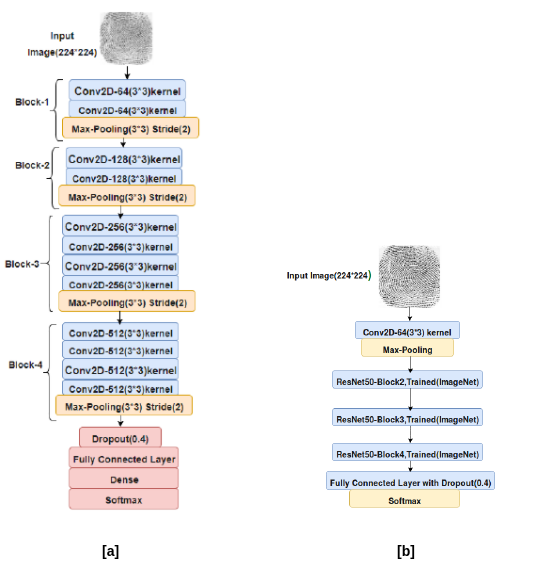
\includegraphics[scale=0.8]{images/ModelDiagram}
\caption{ [a] VGG-19 based shallow network, [b] Resnet50 based deep network.
}\label{fig:figure7}
\end{figure} 

\subsection{Experimantal Analysis}
\label{sec:expAnalysis}

	The proposed two architectures described in the previous section has been tested upon four publicly available benchmark single fingerprint databases viz., (i) FVC2002, (ii) FVC2004 and (iii) FVC2006 (iv) IITD-MOLF and on IITK database which is not publicly available and the largest dataset comprising of more than 40, 000 images so far.
	
	The IITK dataset of single fingerprints consists of 41, 129 images collected using three different types of sensors viz., (i) Futronic (FS88H), (ii)Lumidigm V310 (V31X) and (iii) SecuGen Hamster I. All of them are of same 500 DIP, but the light source and the image size generated is different. All FVC dataset consists of images collected from four different types of sensors. We have trained the proposed model by taking only 10\% of the single finger print images as training set and rest 90\% as testing set, thus adopting a very difficult protocol.
	
	The results are computed for two different testing strategies namely (a) Intra sensor classification (b) Multi sensor classification. The Correct Classification Rate (CCR\%) is computed for performance evaluation, higher the value better is the result


	\begin{itemize}
		\item {Intra-sensor Classification}

		In this type of classification training and testing is performed on images acquired from same type of sensor model. Table~\ref{tab:table1}, indicates the computed performance of two different proposed architectures on various datasets. The main phenomenon that we observed is that we are getting almost same type of CCR(\%) inspite of the fact of using two different kind of varied architectures. This can be attributed to the fact that fingerprint classification problem is a fine grain problem which does not require to learn features at the finest granular level and thus even shallow network is giving remarkable performance
	\end{itemize}

\begin{longtable}[c]{|l|l|l|l|}
\caption{Intra Sensor qualitative performance in CCR(\%) on proposed architectures(DB1 means the images from the first sensor of the
corresponding dataset and same nomenclature is used for other
datasets)}
\label{tab:table1}\\
\hline
Datasets & Sensor Type & Shallow & Deep \\ \hline
\endfirsthead
%
\endhead
%
FVC 2002 & \begin{tabular}[c]{@{}l@{}}DB1\\ DB2\\ DB3\\ DB4\\ Aggregate\end{tabular} & \begin{tabular}[c]{@{}l@{}}100\\ 99.17\\ 100\\ 99.72\\ 99.72\end{tabular} & \begin{tabular}[c]{@{}l@{}}100\\ 96.79\\ 99.72\\ 99.45\\ 98.99\end{tabular} \\ \hline
FVC 2004 & \begin{tabular}[c]{@{}l@{}}DB1\\ DB2\\ DB3\\ DB4\\ Aggregate\end{tabular} & \begin{tabular}[c]{@{}l@{}}100\\ 100\\ 99.85\\ 100\\ 99.96\end{tabular} & \begin{tabular}[c]{@{}l@{}}100\\ 100\\ 93.78\\ 99.17\\ 98.23\end{tabular} \\ \hline
FVC 2006 & \begin{tabular}[c]{@{}l@{}}DB1\\ DB2\\ DB3\\ DB4\\ Aggregate\end{tabular} & \begin{tabular}[c]{@{}l@{}}100\\ 100\\ 100\\ 99.93\\ 99.98\end{tabular} & \begin{tabular}[c]{@{}l@{}}99.87\\ 99.28\\ 99.80\\ 100\\ 99.73\end{tabular} \\ \hline
IITD-MOLF & \begin{tabular}[c]{@{}l@{}}DB1\\ DB2\\ DB3\\ Aggregate\end{tabular} & \begin{tabular}[c]{@{}l@{}}100\\ 100\\ 99.92\\ 99.97\end{tabular} & \begin{tabular}[c]{@{}l@{}}100\\ 100\\ 100\\ 100\end{tabular} \\ \hline
IITK Dataset & \begin{tabular}[c]{@{}l@{}}Futronic\\ Lumidigm\\ SecuGen\\ Aggregate\end{tabular} & \begin{tabular}[c]{@{}l@{}}99.45\\ 100\\ 100\\ 99.82\end{tabular} & \begin{tabular}[c]{@{}l@{}}99.34\\ 100\\ 100\\ 99.78\end{tabular} \\ \hline
\end{longtable}

	\begin{itemize}
		\item \textbf{Multi-sensor Classification}

		In multi-sensor classification, data is fused together from various fingerprint sensors. We did this purposefully in order to check the generalizability of our proposed architectures. We have merged data from all FVC datasets i.e. FVC2002, FVC 2004 and FVC 2006. The combined dataset consists of 13, 063 images resulting from 12 different sensors and trained our network with 12 output neurons. We have trained our proposed model on 1306 images and tested on remaining 11, 757 images (i.e. 10\% training and 90\% testing). Table~\ref{tab:table2} indicates the computed performance in terms of CCR(\%). We have observed that the obtained results are quite remarkable which depicts the high gener alizability of our proposed architectures. In this case also shallow networks are learning discriminative features quite well
	\end{itemize}

\begin{longtable}[c]{|l|l|l|l|}
\caption{Mutli-sensor qualitative performance in CCR(\%) on proposed architectures (here in xDBy: x stands for FVC dataset number and y stands for sensor type of the corresponding dataset)}
\label{tab:table2}\\
\hline
Dataset & Sensor Type & Shallow & Deep \\ \hline
\endfirsthead
%
\endhead
%
FVC Combined & \begin{tabular}[c]{@{}l@{}}2DB1\\ 2DB2\\ 2DB3\\ 2DB4\\ 4DB1\\ 4DB2\\ 4DB3\\ 4DB4\\ 6DB1\\ 6DB2\\ 6DB3\\ 6DB4\\ Aggregate\end{tabular} & \begin{tabular}[c]{@{}l@{}}98.75\\ 97.63\\ 100\\ 99.58\\ 99.31\\ 100\\ 100\\ 100\\ 100\\ 100\\ 99.86\\ 99.80\\ 99.58\end{tabular} & \begin{tabular}[c]{@{}l@{}}99.29\\ 98.37\\ 99.57\\ 99.72\\ 99.16\\ 100\\ 99.40\\ 97.47\\ 100\\ 100\\ 98.56\\ 100\\ 99.29\end{tabular} \\ \hline
\end{longtable}

\subsection{Robustness or Generalization Analysis}
\label{sec:robustGeneralization}
	In order to gain further insights in understanding the effectiveness and generalization of the proposed architecture we introduce some artifacts in the original image in the form of random-noise, rotation and occlusion. All these artifacts are done on a small validation-set comprising of 100 images for each sensor corresponding to IITK single fingerprint dataset.

	\begin{itemize}
		\item \textbf{Rotation}

	In order to check the robustness of the proposed architecture the input fingerprint images have been rotated with different angles and the computed CCR\% is shown in Table~\ref{tab:table3}. It can be inferred from Table~\ref{tab:table3} as we increase the angle of rotation the performance of SecuGen sensor decreases drastically this can be attributed to the non uniformity of the image captured through it as clearly visible from Fig~\ref{fig:figure2}

\begin{longtable}[c]{|l|l|l|l|}
\caption{Rotation qualitative performance in CCR(\%) on validation set for shallow network architecture (here 2, 4, 6, 8 and 15 represents the angle of rotation in clockwise as well as in anti-clockwise direction )}
\label{tab:table3}\\
\hline
Angle & Sensor                                                                & VGG                                                     & Resnet                                                   \\ \hline
\endfirsthead
%
\endhead
%
2     & \begin{tabular}[c]{@{}l@{}}Futronic\\ Lumidigm\\ SecuGen\end{tabular} & \begin{tabular}[c]{@{}l@{}}99\\ 100\\ 94.5\end{tabular} & \begin{tabular}[c]{@{}l@{}}100\\ 100\\ 100\end{tabular}  \\ \hline
4     & \begin{tabular}[c]{@{}l@{}}Futronic\\ Lumidigm\\ SecuGen\end{tabular} & \begin{tabular}[c]{@{}l@{}}99\\ 100\\ 84.5\end{tabular} & \begin{tabular}[c]{@{}l@{}}100\\ 100\\ 100\end{tabular}    \\ \hline
6     & \begin{tabular}[c]{@{}l@{}}Futronic\\ Lumidigm\\ SecuGen\end{tabular} & \begin{tabular}[c]{@{}l@{}}99\\ 100\\ 80\end{tabular}   & \begin{tabular}[c]{@{}l@{}}100\\ 100\\ 100\end{tabular}  \\ \hline
8     & \begin{tabular}[c]{@{}l@{}}Futronic\\ Lumidigm\\ SecuGen\end{tabular} & \begin{tabular}[c]{@{}l@{}}99\\ 100\\ 76\end{tabular}   & \begin{tabular}[c]{@{}l@{}}100\\ 100\\ 95.8\end{tabular} \\ \hline
\end{longtable}

		\item \textbf{Occlusion}

	In order to test whether our proposed architecture is invariant to occlusion or not. We consider a patch of 90 X 90 in the input image and randomly occluded some percentage of pixels in it. The results in terms of CCR\% has been shown in Table~\ref{tab:table4}. Surprisingly it can be inferred from Table~\ref{tab:table4} that on increasing the occlusion in the image the performance of the network is not deteriorating. This abnormal behaviour compel us to think what exactly our network is learning.

\begin{longtable}[c]{|l|l|l|l|}
\caption{Occlusion qualitative performance in CCR(\%) on validation set for shallow network architecture (here 1\%,5\% and 10\% are the percentage of pixels occluded in a region of 90 X 90 patch )
}
\label{tab:table4}\\
\hline
Percentage & Sensor                                                                & VGG                                                       & Resnet                                                     \\ \hline
\endfirsthead
%
\endhead
%
1          & \begin{tabular}[c]{@{}l@{}}Futronic\\ Lumidigm\\ SecuGen\end{tabular} & \begin{tabular}[c]{@{}l@{}}100\\ 99.8\\ 99.8\end{tabular} & \begin{tabular}[c]{@{}l@{}}99.8\\ 100\\ 100\end{tabular}   \\ \hline
5          & \begin{tabular}[c]{@{}l@{}}Futronic\\ Lumidigm\\ SecuGen\end{tabular} & \begin{tabular}[c]{@{}l@{}}100\\ 99.6\\ 100\end{tabular}  & \begin{tabular}[c]{@{}l@{}}100\\ 100\\ 100\end{tabular}    \\ \hline
10         & \begin{tabular}[c]{@{}l@{}}Futronic\\ Lumidigm\\ SecuGen\end{tabular} & \begin{tabular}[c]{@{}l@{}}100\\ 99.2\\ 99.2\end{tabular} & \begin{tabular}[c]{@{}l@{}}99.4\\ 99.8\\ 98.6\end{tabular} \\ \hline
15         & \begin{tabular}[c]{@{}l@{}}Futronic\\ Lumidigm\\ SecuGen\end{tabular} & \begin{tabular}[c]{@{}l@{}}100\\ 98.2\\ 98.2\end{tabular} & \begin{tabular}[c]{@{}l@{}}99.6\\ 100\\ 98\end{tabular}    \\ \hline
\end{longtable}

		\item \textbf{Random Noise}

	In real life scenarios it is very difficult to get a perfect condition. Most of the time we end up with noise affecting our ideal conditions. In such cases it is essential that our architecture is robust for noise upto certain range. Table~\ref{tab:table5} shows the result of adding random noise to our validation test data. It can be infered from Table~\ref{tab:table5} that on increasing the random noise the performance of the Lumidigm sensor is decaying to a large extent. As it is clearly evident from Table~\ref{fig:figure2} that the Lumidigm sensor captured image is highly uniform in texture, so any small alteration or artifact in its texture greatly affects our network performance.

\begin{longtable}[c]{|l|l|l|l|}
\caption{ Random noise qualitative performance in CCR(\%) on validation set for shallow network architecture (here 0.01\%, 0.05\%, 0.1\% are the percentage of the random noise inserted in the input image of size 224 ∗ 224 )
}
\label{tab:table5}\\
\hline
Percentage & Sensor                                                                & VGG                                                   & Resnet                                                   \\ \hline
\endfirsthead
%
\endhead
%
0.01       & \begin{tabular}[c]{@{}l@{}}Futronic\\ Lumidigm\\ SecuGen\end{tabular} & \begin{tabular}[c]{@{}l@{}}99\\ 100\\ 99\end{tabular} & \begin{tabular}[c]{@{}l@{}}100\\ 100\\ 100\end{tabular}  \\ \hline
0.05       & \begin{tabular}[c]{@{}l@{}}Futronic\\ Lumidigm\\ SecuGen\end{tabular} & \begin{tabular}[c]{@{}l@{}}99\\ 94\\ 98\end{tabular}  & \begin{tabular}[c]{@{}l@{}}100\\ 97.8\\ 100\end{tabular} \\ \hline
0.1        & \begin{tabular}[c]{@{}l@{}}Futronic\\ Lumidigm\\ SecuGen\end{tabular} & \begin{tabular}[c]{@{}l@{}}99\\ 50\\ 98\end{tabular}  & \begin{tabular}[c]{@{}l@{}}100\\ 85.6\\ 100\end{tabular} \\ \hline
\end{longtable}


	\end{itemize}

\subsection{Layer Specific Feature Analysis}
\label{sec:layerSpecificFeature}

	As it is clearly evident from Table~\ref{tab:table5} that on increasing the amount of occlusion on our input images the performance of our proposed network is not degrading. This compels us to think some interesting questions: like what exactly our network is learning? Is there something wrong in its learning? Is there any kind of prestidigitation in our network? In order to answer these questions we try to visualize the feature maps learned by different layers of our proposed shallow network. For visualizing the feature-maps we took the SecuGen sensor of IIIT-K single fingerprint images. Part (a) of Fig~\ref{fig:figure8} shows the features learned by our proposed shallow network. It is clearly evident from the Fig~\ref{fig:figure8} , that initial convolutional layers are learning general specific features, while as we go deeper and deeper more sensor specific features, localized and sparse features are learned. It can be observed in Part (a) of Fig~\ref{fig:figure8} that layer 3 and layer 6 are trying to understand the textual patterns of the image, but as we move deeper in the network like in layer 9 and layer 14 more emphasis is given to learn the shape and the background of the image rather than its textual patterns. By observing this we realize that our network is smart enough instead of learning finer granular level discriminative information to distinguish between different sensors it learned the background and shape of the image instead of its textual features.

	This could be the main reason for the exceptionally high performance of the network in case of occluded images. In order to prove it we did another set of experimentation in this we crop an input image from the middle in the size of 90 X 90 patch and paste it over a white background. By doing this we have forcefully made the background of all the images same, in-order to force our network to learn textual features instead of background. It is clearly evident from Fig~\ref{fig:figure8} that now our network is learning textual patterns instead of background. It is also proved by the results that we obtained after adding occlusion on this set of images

\begin{figure}[htbp]
\centering
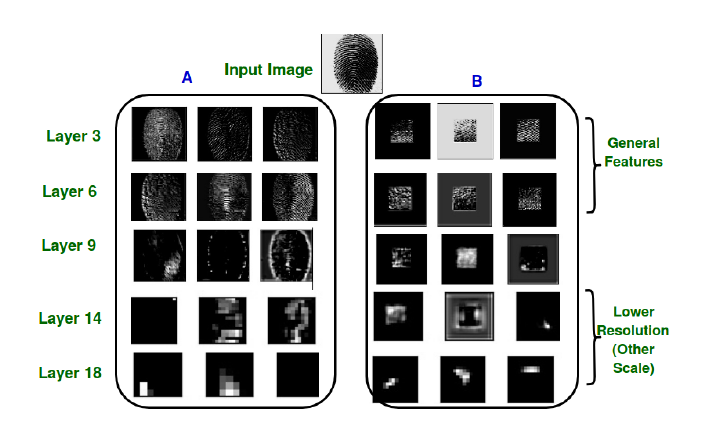
\includegraphics[scale=1]{images/FeatureAnalysis}
\caption{ Comparative Feature Analysis.
}\label{fig:figure8}
\end{figure} 


\end{document}
 
 
 
